% blog-title: Why Bandits Matter
% blog-date: 2026-06-15
% blog-description: Sequential decision-making beyond supervised learning: feedback, regret, optimism, and Thompson sampling in one reproducible note.
% blog-lang: en

\documentclass[en,nofont,11pt]{elegantbook}

\title{Why Bandits Matter}
\subtitle{Sequential Decision-Making Beyond Supervised Learning}
\author{Tang}
\institute{Tang's Machine Learning Blog}
\date{2026-06-15}
\version{1.0.0}
\bioinfo{Topic}{Bandits, Online Learning, Sequential Decision-Making}
\cover{assets/blog-cover.jpg}

\usepackage{fontspec}
\ifdefined\setCJKmainfont
\else
  \usepackage[UTF8,scheme=plain,fontset=none]{ctex}
\fi
\usepackage{xcolor}
\usepackage{listings}
\usepackage{float}
\usepackage{tcolorbox}
\tcbuselibrary{breakable, listings, skins}
\usetikzlibrary{arrows.meta,positioning,calc,decorations.pathmorphing,decorations.pathreplacing,fit,backgrounds,patterns,shapes.geometric}

\IfFontExistsTF{Microsoft YaHei}{
  \setCJKmainfont{Microsoft YaHei}
  \setCJKsansfont{Microsoft YaHei}
  \setCJKmonofont{Microsoft YaHei UI}
}{
  \IfFontExistsTF{Noto Serif CJK SC}{
    \setCJKmainfont{Noto Serif CJK SC}
    \setCJKsansfont{Noto Sans CJK SC}
    \setCJKmonofont{Noto Sans Mono CJK SC}
  }{}
}

\definecolor{blogAccent}{HTML}{1F6F8B}
\definecolor{blogInk}{HTML}{172026}
\definecolor{blogCodeBg}{HTML}{F5F7F8}
\definecolor{blogCodeBorder}{HTML}{D6E2E8}
\definecolor{blogKeyword}{HTML}{B23A48}
\definecolor{blogString}{HTML}{287D4F}
\definecolor{blogComment}{HTML}{687783}

\lstdefinestyle{blogcode}{
  basicstyle=\ttfamily\small,
  keywordstyle=\bfseries\color{blogKeyword},
  stringstyle=\color{blogString},
  commentstyle=\itshape\color{blogComment},
  numberstyle=\scriptsize\color{blogComment},
  numbers=left,
  numbersep=8pt,
  showstringspaces=false,
  breaklines=true,
  tabsize=2,
  columns=fullflexible,
  keepspaces=true
}

\newtcblisting{codeblock}[2][]{
  listing only,
  breakable,
  enhanced,
  colback=blogCodeBg,
  colframe=blogCodeBorder,
  arc=2mm,
  boxrule=0.4pt,
  left=6mm,
  right=2mm,
  top=1mm,
  bottom=1mm,
  listing options={style=blogcode, language=#2},
  #1
}

\hypersetup{
  colorlinks=true,
  linkcolor=blogAccent,
  urlcolor=blogAccent,
  citecolor=blogAccent
}

\addbibresource{tex/bandits-references.bib}

\definecolor{softgreen}{HTML}{E8F5E9}
\definecolor{softred}{HTML}{FFF1F2}
\definecolor{softblue}{HTML}{EAF2FF}
\definecolor{softorange}{HTML}{FFF7ED}
\definecolor{softpurple}{HTML}{F3E8FF}
\definecolor{softyellow}{HTML}{FFFCEB}
\definecolor{banditPurple}{HTML}{7C3AED}
\definecolor{blogblue}{HTML}{7A3D25}
\definecolor{blogorange}{HTML}{B23A48}
\colorlet{banditBlue}{blogAccent}
\colorlet{banditOrange}{blogKeyword}

\newtcolorbox{takeawaybox}{
  breakable,
  colback=blogCodeBg,
  colframe=banditBlue,
  boxrule=0.6pt,
  arc=2pt,
  left=8pt,
  right=8pt,
  top=8pt,
  bottom=8pt,
  title=Takeaway,
  fonttitle=\bfseries
}

\newtcolorbox{storybox}[1]{
  breakable,
  colback=softblue,
  colframe=banditBlue,
  boxrule=0.65pt,
  arc=2pt,
  left=8pt,
  right=8pt,
  top=8pt,
  bottom=8pt,
  title={#1},
  fonttitle=\bfseries
}

\newtcolorbox{plainbox}[1]{
  breakable,
  colback=softyellow,
  colframe=banditOrange,
  boxrule=0.6pt,
  arc=2pt,
  left=8pt,
  right=8pt,
  top=8pt,
  bottom=8pt,
  title={#1},
  fonttitle=\bfseries
}

\newtcolorbox{derivationbox}[1]{
  breakable,
  colback=white,
  colframe=banditBlue,
  boxrule=0.55pt,
  arc=2pt,
  left=8pt,
  right=8pt,
  top=6pt,
  bottom=6pt,
  title={#1},
  fonttitle=\bfseries\itshape
}

\newtcolorbox{proofbox}[1]{
  breakable,
  colback=white,
  colframe=banditPurple,
  boxrule=0.55pt,
  arc=2pt,
  left=8pt,
  right=8pt,
  top=6pt,
  bottom=6pt,
  title={#1},
  fonttitle=\bfseries\itshape
}

\newtcolorbox{researchbox}[1]{
  breakable,
  colback=softpurple,
  colframe=banditPurple,
  boxrule=0.65pt,
  arc=2pt,
  left=8pt,
  right=8pt,
  top=8pt,
  bottom=8pt,
  title={#1},
  fonttitle=\bfseries
}

\newcommand{\E}{\mathbb{E}}
\newcommand{\Pp}{\mathbb{P}}
\newcommand{\R}{\mathbb{R}}
\newcommand{\ind}{\mathbf{1}}
\newcommand{\KL}{\mathrm{KL}}
\newcommand{\Ber}{\mathrm{Ber}}
\newcommand{\Beta}{\mathrm{Beta}}
\newcommand{\Normal}{\mathcal{N}}
\newcommand{\GP}{\mathcal{GP}}
\newcommand{\calA}{\mathcal{A}}
\newcommand{\calF}{\mathcal{F}}
\newcommand{\calH}{\mathcal{H}}
\newcommand{\calX}{\mathcal{X}}
\newcommand{\calD}{\mathcal{D}}
\providecommand{\argmax}{\mathop{\mathrm{argmax}}}
\providecommand{\argmin}{\mathop{\mathrm{argmin}}}
\providecommand{\Reg}{\operatorname{Reg}}

\begin{document}
\maketitle
\frontmatter
\tableofcontents
\mainmatter
\chapter*{Before the First Formula}
\addcontentsline{toc}{chapter}{Before the First Formula}

The first question in a learning problem is not ``which model should we use?'' It is more primitive:

\begin{quote}
Where did the data come from?
\end{quote}

In supervised learning, the data usually arrive as a table. Someone has already collected the inputs and labels. The learner may be clever or foolish, but the table is there.

In bandit learning, the table is not there. The learner helps create it. Each action asks the world one question, and the world answers only that question.

This is the whole difference. A bandit algorithm is not merely predicting from data. It is choosing which data it will get to see.

\begin{plainbox}{The shortest useful definition}
A bandit problem is learning by trying one option at a time, while never seeing what would have happened under the options not tried.
\end{plainbox}

That sentence is enough to begin. The mathematics enters only because we want to measure how costly this kind of learning is, and how a good algorithm keeps the cost under control.

A helpful mental picture is an ordinary recommendation slot. At 8:00 a.m., the system chooses one item to show. A user clicks or does not click. The system sees the outcome of the shown item, but it does not see the click outcomes of the hidden items. Tomorrow it must choose again, using yesterday's incomplete evidence.

This example is not special. The same shape appears when a teacher chooses one hint for a student, a doctor chooses one treatment, a lab chooses one experiment, or a prompt-selection system chooses one prompt for a language model. In all cases, the learner receives feedback from the chosen action, not from the unchosen alternatives.

The goal of this note is to keep that simple picture visible while building the main formulas. The style follows a useful tradition in modern bandit writing: start from the feedback pattern, use examples to make the pressure of the problem visible, and introduce proof machinery only when it pays rent. Lattimore and Szepesvari describe their book as mathematically focused but not a traditional chain of lemmas and theorems; they emphasize guiding principles, intuition, and depth over formal display \cite{lattimore2020bandit}. That is the standard I have in mind here.

\begin{figure}[h]
\centering
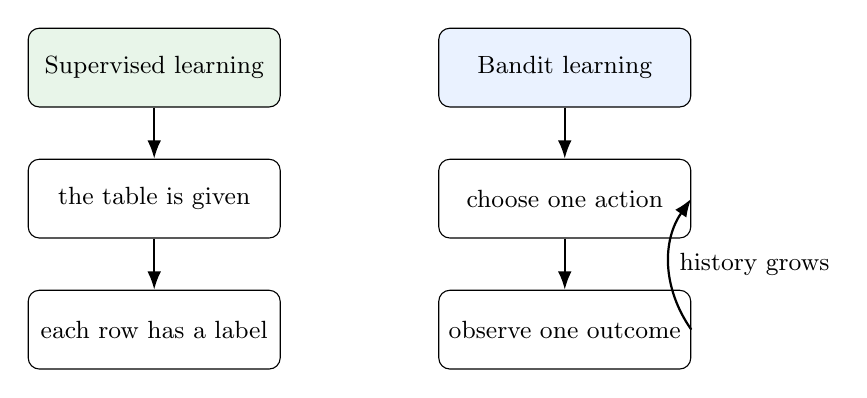
\begin{tikzpicture}[font=\small, node distance=1.15cm, >=Latex]
  \tikzstyle{box}=[draw, rounded corners, align=center, minimum width=3.2cm, minimum height=1.0cm, fill=white]
  \node[box, fill=softgreen] (sup) {Supervised learning};
  \node[box, below=0.65cm of sup] (supdata) {the table is given};
  \node[box, below=0.65cm of supdata] (suplabel) {each row has a label};
  \draw[->, thick] (sup) -- (supdata);
  \draw[->, thick] (supdata) -- (suplabel);

  \node[box, fill=softblue, right=2.0cm of sup] (ban) {Bandit learning};
  \node[box, below=0.65cm of ban] (banact) {choose one action};
  \node[box, below=0.65cm of banact] (banobs) {observe one outcome};
  \draw[->, thick] (ban) -- (banact);
  \draw[->, thick] (banact) -- (banobs);
  \draw[->, thick, bend left=35] (banobs.east) to node[right]{history grows} (banact.east);
\end{tikzpicture}
\caption{Supervised learning starts from a table. Bandit learning builds a table by acting.}
\end{figure}

% ------------------------------------------------------------
\chapter{The First Object Is the Feedback}

\section{Do not start with a tuple}

A common weak opening is to define a bandit problem as a list of symbols. That is technically correct and pedagogically backwards. The first object is not a tuple. The first object is the feedback.

Suppose there are several actions. At a given moment, you choose one. The world returns one number. The other numbers remain unobserved.

Only now do the symbols become useful. Let
\[
A_t
\]
be the action chosen at time $t$, and let
\[
X_t(A_t)
\]
be the reward observed after choosing it. If $a\neq A_t$, then $X_t(a)$ is not observed.

\begin{derivationbox}{The feedback pattern}
\[
\begin{aligned}
\text{choose }A_t
&\quad\Longrightarrow\quad \text{observe }X_t(A_t),\\
\text{do not choose }a
&\quad\Longrightarrow\quad \text{do not observe }X_t(a).
\end{aligned}
\]
\end{derivationbox}

The second line is the source of almost everything in bandit theory. The missing outcome is not a nuisance. It is the problem.

\section{The missing column}

Imagine two possible actions, $A$ and $B$. For a single user, there are two potential outcomes:
\[
X(A),\qquad X(B).
\]
One says what would happen if we chose $A$. The other says what would happen if we chose $B$. We can reveal only one.

\[
\begin{array}{c|cc|c}
\text{chosen action} & X(A) & X(B) & \text{observed outcome}\\
\midrule
A & \text{visible} & \text{hidden} & X(A)\\
B & \text{hidden} & \text{visible} & X(B)
\end{array}
\]

A supervised-learning dataset tries to fill the label column for every example. A bandit dataset has a hole in every row. The hole is exactly where the unchosen actions would have been.

\begin{plainbox}{A useful plain-language test}
If after acting you can ask, ``what would have happened if I had chosen differently?'' and the data cannot answer, you are in bandit territory.
\end{plainbox}

\section{Why bad actions damage future data}

In supervised learning, a bad prediction is painful, but the label still arrives. In bandit learning, a bad action can also damage the learner's future evidence.

If an algorithm always chooses the currently popular item, it keeps collecting data about that item. The less popular item may remain uncertain forever. The learner is not only using biased data; it is generating the bias.

This is why bandit algorithms need exploration. Exploration is not curiosity for its own sake. It is the repair mechanism for missing feedback.

\begin{figure}[h]
\centering
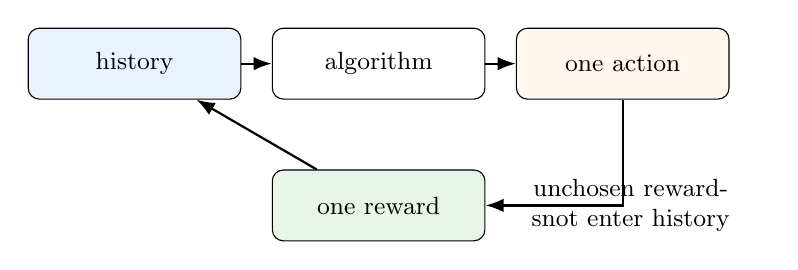
\begin{tikzpicture}[font=\small, >=Latex]
  \node[draw, rounded corners, fill=softblue, align=center, minimum width=2.7cm, minimum height=0.9cm] (hist) at (0,0) {history};
  \node[draw, rounded corners, fill=white, align=center, minimum width=2.7cm, minimum height=0.9cm] (alg) at (3.1,0) {algorithm};
  \node[draw, rounded corners, fill=softorange, align=center, minimum width=2.7cm, minimum height=0.9cm] (act) at (6.2,0) {one action};
  \node[draw, rounded corners, fill=softgreen, align=center, minimum width=2.7cm, minimum height=0.9cm] (rew) at (3.1,-1.8) {one reward};
  \draw[->, thick] (hist) -- (alg);
  \draw[->, thick] (alg) -- (act);
  \draw[->, thick] (act) |- (rew);
  \draw[->, thick] (rew) -- (hist);
  \node[align=center, text width=3.3cm] at (6.3,-1.8) {unchosen rewards\do not enter history};
  \draw[dashed, thick] (6.2,-0.55) -- (6.2,-1.35);
\end{tikzpicture}
\caption{The learner's action controls the next piece of data. This feedback loop is the main difference from ordinary supervised learning.}
\end{figure}


% ------------------------------------------------------------
\chapter{A Small Experiment Before More Theory}

\section{The same world, two ways to learn}

Before adding more probability, it is useful to run a tiny experiment. The point is not to make a benchmark. The point is to make the feedback pattern visible.

There are three arms. You may think of them as three possible thumbnails, three prompts, or three treatments in a toy clinical example. Their click probabilities are
\[
\mu_1=0.10,\qquad \mu_2=0.12,\qquad \mu_3=0.16.
\]
Arm $3$ is best, but the learner does not know this.

We compare four learners in exactly the same world.

\begin{itemize}
  \item \textbf{Full-feedback learner.} It chooses one arm but observes the reward of every arm. This is the supervised-learning spirit: labels are supplied by the data-collection process rather than purchased one action at a time.
  \item \textbf{Greedy bandit.} It tries each arm once, then always chooses the arm with the largest observed average.
  \item \textbf{UCB.} It chooses the arm with the largest empirical mean plus an uncertainty bonus.
  \item \textbf{Thompson sampling.} It samples a plausible click rate for every arm from its posterior and chooses the arm whose sampled value is largest.
\end{itemize}

The full-feedback learner is not meant to be a general supervised-learning algorithm. It is the cleanest possible full-information analogue. Its purpose is to isolate the difference between seeing all labels and seeing only the label of the action we picked.

\begin{plainbox}{What the experiment should reveal}
If every round gives labels for all arms, learning is mostly estimation. If every round gives only one label, learning is also data acquisition. The learner must decide which uncertainty is worth reducing.
\end{plainbox}

\section{The algorithms in code}

The code below is deliberately plain. No library hides the learning rule. Each algorithm keeps a few counters and chooses an arm.

\begin{codeblock}[title={A minimal reproducible simulation for full feedback, greedy bandits, UCB, and Thompson sampling.}]{Python}
import numpy as np

def run_once(p, T, rng):
    K = len(p)
    best = np.max(p)
    regret = {"full": [], "greedy": [], "ucb": [], "ts": []}

    # 1. Full feedback: choose one arm, observe all arms.
    sums = np.zeros(K)
    counts = np.zeros(K)
    for t in range(T):
        if t < K:
            a = t
        else:
            a = np.argmax(sums / np.maximum(counts, 1))
        regret["full"].append(best - p[a])

        rewards_all = rng.binomial(1, p)   # the full row is visible
        sums += rewards_all
        counts += 1

    # 2. Greedy bandit: observe only the chosen arm.
    sums = np.zeros(K)
    counts = np.zeros(K)
    for t in range(T):
        if t < K:
            a = t
        else:
            a = np.argmax(sums / np.maximum(counts, 1))
        r = rng.binomial(1, p[a])          # only this reward is visible
        regret["greedy"].append(best - p[a])
        sums[a] += r
        counts[a] += 1

    # 3. UCB: empirical mean plus an uncertainty bonus.
    sums = np.zeros(K)
    counts = np.zeros(K)
    for t in range(T):
        if t < K:
            a = t
        else:
            mean = sums / counts
            radius = np.sqrt(2 * np.log(t + 1) / counts)
            a = np.argmax(mean + radius)
        r = rng.binomial(1, p[a])
        regret["ucb"].append(best - p[a])
        sums[a] += r
        counts[a] += 1

    # 4. Thompson sampling for Bernoulli rewards.
    alpha = np.ones(K)
    beta = np.ones(K)
    for t in range(T):
        sample = rng.beta(alpha, beta)
        a = np.argmax(sample)
        r = rng.binomial(1, p[a])
        regret["ts"].append(best - p[a])
        alpha[a] += r
        beta[a] += 1 - r

    return {name: np.cumsum(vals) for name, vals in regret.items()}
\end{codeblock}

Read the code slowly. The full-feedback learner has the line
\[
\texttt{rewards\_all = rng.binomial(1, p)}.
\]
That line gives it a whole row of labels. The bandit algorithms have the line
\[
\texttt{r = rng.binomial(1, p[a])}.
\]
That line gives them only the chosen label. The difference between these two lines is the difference between supervised-style feedback and bandit feedback.

\section{What the code produces}

I ran the experiment for $T=2000$ rounds and averaged over $400$ independent runs. The table reports the final cumulative regret and the average number of pulls of each arm.

\begin{table}[H]
\centering
\small
\begin{tabular}{lrrrr}
\toprule
Algorithm & Final regret & Pulls of arm 1 & Pulls of arm 2 & Pulls of arm 3 \\
\midrule
Full feedback & $4.57$ & $26.2$ & $74.8$ & $1899.0$ \\
Greedy bandit & $98.08$ & $1504.0$ & $196.0$ & $300.0$ \\
UCB & $49.81$ & $448.7$ & $572.2$ & $979.1$ \\
Thompson sampling & $21.23$ & $160.6$ & $289.8$ & $1549.5$ \\
\bottomrule
\end{tabular}
\caption{Average behavior over 400 runs with true means $(0.10,0.12,0.16)$ and horizon $T=2000$.}
\end{table}

The numbers tell the story without any theorem.

The full-feedback learner rapidly finds the best arm because every round teaches it about every arm. Greedy often gets trapped by early noise. UCB keeps checking uncertain arms because uncertainty itself becomes part of the index. Thompson sampling explores in a softer way: an arm is tried when its posterior still gives it a plausible chance of being best.

\begin{figure}[H]
\centering

\includegraphics[width=0.86\linewidth]{assets/bandits/regret_curves.pdf}
\caption{Average cumulative regret. The greedy bandit can pay a large price for believing early noise. UCB and Thompson sampling reduce this cost by making uncertainty operational.}
\end{figure}

\begin{figure}[H]
\centering

\includegraphics[width=0.86\linewidth]{assets/bandits/pull_counts.pdf}
\caption{Average pull counts. The best arm is arm $3$. The greedy learner often spends many rounds on the wrong arm; the sampling and optimism-based methods move probability mass toward the best arm while still collecting evidence.}
\end{figure}

\section{The lesson hidden in the experiment}

A supervised learner can be viewed as a reader of a completed table. A bandit learner is a writer of an incomplete table. This makes a qualitative difference.

\begin{derivationbox}{The one-line difference}
\[
\begin{aligned}
\text{full feedback:}&\qquad (X_t(1),X_t(2),X_t(3))\text{ is observed},\\
\text{bandit feedback:}&\qquad X_t(A_t)\text{ is observed, and }X_t(a)\text{ for }a\neq A_t\text{ is missing}.
\end{aligned}
\]
\end{derivationbox}

Now the later formulas have a concrete object to explain. Regret measures the cost of not knowing the best arm. Confidence intervals explain why UCB does not blindly trust early averages. Posterior sampling explains why Bayesian uncertainty can be converted into action.

% ------------------------------------------------------------
\chapter{Probability, Introduced Only When Needed}

\section{A reward is a number we have not seen yet}

Probability can sound abstract when introduced as a formal system. In bandits, its first role is modest: it gives language for numbers we have not seen yet.

Before an item is shown, its click outcome is unknown. After it is shown, the outcome becomes a number. We model the before-state by a random variable.

For a click/no-click reward,
\[
X=\begin{cases}
1, & \text{click},\\
0, & \text{no click}.
\end{cases}
\]
If the click probability is $\mu$, then
\[
\Pp(X=1)=\mu,
\qquad
\Pp(X=0)=1-\mu.
\]
The average value of this random reward is
\[
\begin{aligned}
\E[X]
&=1\cdot \Pp(X=1)+0\cdot \Pp(X=0)\\
&=1\cdot \mu+0\cdot(1-\mu)\\
&=\mu.
\end{aligned}
\]

So in a click model, the mean reward is simply the click probability.

\section{The sample average is a noisy ruler}

If we try the same arm $n$ times, we see rewards
\[
Y_1,Y_2,\ldots,Y_n.
\]
The empirical mean is
\[
\widehat\mu_n=\frac{1}{n}\sum_{i=1}^n Y_i.
\]
This is the observed click rate. It is our ruler for the unknown mean $\mu$.

But the ruler is noisy. If a thumbnail has true click probability $0.10$, it can still receive $2$ clicks in $10$ trials or $0$ clicks in $10$ trials. Small samples wobble.

The first probability question is therefore:

\begin{quote}
How far can the observed average be from the true average?
\end{quote}

For bounded rewards in $[0,1]$, Hoeffding's inequality says that large errors become exponentially unlikely:
\[
\Pp\left(\left|\widehat\mu_n-\mu\right|\geq r\right)
\leq
2\exp(-2nr^2).
\]

This line is not meant to be memorized as a magic spell. Read it from right to left:
\[
\begin{array}{ccl}
 n \text{ grows} &\Longrightarrow& \exp(-2nr^2) \text{ shrinks},\\
 r \text{ grows} &\Longrightarrow& \exp(-2nr^2) \text{ shrinks}.
\end{array}
\]
More data makes a fixed error less likely. A larger error is also less likely.

\section{Turning a tail bound into an error bar}

Algorithms usually want an error bar. That means choosing $r$ so that the probability of error is at most a small number $\delta$:
\[
\Pp\left(\left|\widehat\mu_n-\mu\right|\geq r\right)
\leq \delta.
\]
Hoeffding gives the sufficient condition
\[
2\exp(-2nr^2)=\delta.
\]
Solve this slowly:

\begin{derivationbox}{From Hoeffding to a confidence radius}
\[
\begin{aligned}
2\exp(-2nr^2)&=\delta\\
\exp(-2nr^2)&=\frac{\delta}{2}\\
\log\left(\exp(-2nr^2)\right)&=\log\left(\frac{\delta}{2}\right)\\
-2nr^2&=\log\left(\frac{\delta}{2}\right)\\
2nr^2&=\log\left(\frac{2}{\delta}\right)\\
r^2&=\frac{\log(2/\delta)}{2n}\\
r&=\sqrt{\frac{\log(2/\delta)}{2n}}.
\end{aligned}
\]
\end{derivationbox}

Thus a clean error bar is
\[
\left|\widehat\mu_n-\mu\right|
\leq
\sqrt{\frac{\log(2/\delta)}{2n}}
\]
with probability at least $1-\delta$.

\begin{plainbox}{The idea behind the formula}
An arm tried only a few times deserves a wide error bar. An arm tried many times deserves a narrow one. UCB is built from exactly this sentence.
\end{plainbox}

\begin{figure}[h]
\centering
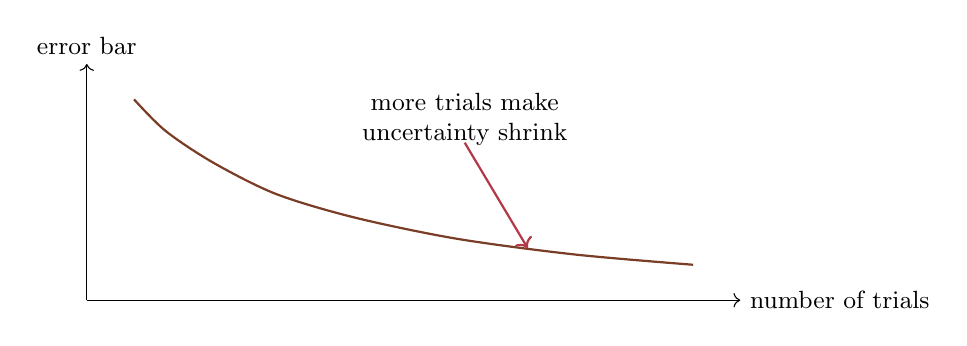
\begin{tikzpicture}[font=\small]
  \draw[->] (0,0) -- (8.3,0) node[right]{number of trials};
  \draw[->] (0,0) -- (0,3.0) node[above]{error bar};
  \draw[thick, blogblue, smooth] plot coordinates {(0.6,2.55) (1.0,2.15) (1.6,1.75) (2.4,1.35) (3.4,1.05) (4.7,0.78) (6.2,0.58) (7.7,0.45)};
  \node[align=center, text width=4.1cm] at (4.8,2.3) {more trials\ make uncertainty shrink};
  \draw[->, thick, blogorange] (4.8,2.0) -- (5.6,0.66);
\end{tikzpicture}
\caption{The confidence radius shrinks like $1/\sqrt{n}$. This shrinking error bar is the engine inside UCB.}
\end{figure}

\section{The union bound is not mysterious}

Many proofs need a statement to hold for many arms and many times. We first control one error event, then combine many such controls.

The only tool needed is the union bound:
\[
\Pp(E_1\cup E_2\cup\cdots\cup E_m)
\leq
\Pp(E_1)+\Pp(E_2)+\cdots+\Pp(E_m).
\]

Why is this true? If two alarms can ring, the chance that at least one rings cannot exceed the sum of their separate chances. The sum may double-count worlds where both alarms ring, so it is an upper bound.

For two events, the exact identity is
\[
\Pp(E_1\cup E_2)
=
\Pp(E_1)+\Pp(E_2)-\Pp(E_1\cap E_2).
\]
Since probabilities are nonnegative,
\[
\Pp(E_1\cap E_2)\geq 0,
\]
so
\[
\Pp(E_1\cup E_2)
\leq
\Pp(E_1)+\Pp(E_2).
\]
For many events, repeat the same idea.

\section{History means what the learner already knows}

Bandit data are adaptive: today's action depends on yesterday's observations. To talk about this without mysticism, we use the word history.

Let $\calF_t$ denote everything known before choosing at time $t$:
\[
\calF_t=\{A_1,X_1(A_1),\ldots,A_{t-1},X_{t-1}(A_{t-1})\}.
\]
An algorithm chooses $A_t$ using this history. Then the new reward arrives and the history grows.

Conditional probability simply means probability after opening the notebook:
\[
\Pp(\text{event}\mid \calF_t)
=
\text{probability of the event given the current notebook}.
\]

\begin{plainbox}{A nontechnical reading of $\calF_t$}
The symbol $\calF_t$ is not there to impress the reader. It means the notebook of everything the learner has seen so far.
\end{plainbox}

This is enough probability for the first bandit algorithms: random rewards, means, sample averages, error bars, union bounds, and history.

% ------------------------------------------------------------
\chapter{Regret Is the Price of Learning}

\section{The meaning before the formula}

A bandit learner must sometimes choose an action that may not be best, because otherwise it may never learn what is best. The cost of these imperfect choices is called regret.

Think of regret as the price paid for not already knowing the best action. If the best thumbnail would have produced a $10\%$ click rate and the chosen thumbnail has an $8\%$ click rate, the expected loss for that decision is $2\%$ of a click.

This does not mean exploration is bad. Exploration is often the only way to stop making the same comfortable mistake. Regret is not a moral judgment. It is accounting.

\section{Now the notation earns its place}

Suppose there are $K$ arms. Arm $a$ has mean reward
\[
\mu_a=\E[X(a)].
\]
The best mean is
\[
\mu_* = \max_{1\leq a\leq K}\mu_a.
\]
If the learner chooses $A_t$, then the expected loss at that time is
\[
\mu_* - \mu_{A_t}.
\]
Adding over $T$ rounds gives pseudo-regret:
\[
\Reg_T=\sum_{t=1}^T(\mu_* - \mu_{A_t}).
\]

This compares the learner with the best fixed arm, not with a magical oracle that knows every random outcome in advance.

\section{The key decomposition}

For each arm define its gap
\[
\Delta_a=\mu_* - \mu_a,
\]
and define the number of times arm $a$ is played by
\[
N_a(T)=\sum_{t=1}^T \ind\{A_t=a\}.
\]
The indicator $\ind\{A_t=a\}$ is just a switch:
\[
\ind\{A_t=a\}=\begin{cases}
1,& A_t=a,\\
0,& A_t\neq a.
\end{cases}
\]

Now decompose regret:

\begin{derivationbox}{Regret as gap times count}
\[
\begin{aligned}
\Reg_T
&=\sum_{t=1}^T(\mu_* - \mu_{A_t})\\
&=\sum_{t=1}^T\sum_{a=1}^K(\mu_* - \mu_a)\ind\{A_t=a\}\\
&=\sum_{a=1}^K(\mu_* - \mu_a)\sum_{t=1}^T\ind\{A_t=a\}\\
&=\sum_{a=1}^K\Delta_a N_a(T).
\end{aligned}
\]
\end{derivationbox}

This formula is the first serious piece of bandit analysis. It says that a bad arm hurts in two ways: how bad it is, and how often it is played.

\section{Checking the switch by hand}

Suppose that at time $t$ the algorithm chose arm $j$. Then exactly one indicator is equal to $1$:
\[
\ind\{A_t=j\}=1,
\qquad
\ind\{A_t=a\}=0\quad(a\neq j).
\]
Therefore
\[
\begin{aligned}
\sum_{a=1}^K(\mu_* - \mu_a)\ind\{A_t=a\}
&=(\mu_* - \mu_1)\ind\{j=1\}+\cdots+(\mu_* - \mu_K)\ind\{j=K\}\\
&=0+\cdots+0+(\mu_* - \mu_j)+0+\cdots+0\\
&=\mu_* - \mu_j\\
&=\mu_* - \mu_{A_t}.
\end{aligned}
\]

No probability is being used here. It is bookkeeping.

\section{Taking expectation}

The count $N_a(T)$ is random because the algorithm's choices depend on random rewards. Its expectation is easy to interpret.

For any event $E$,
\[
\E[\ind\{E\}]
=1\cdot\Pp(E)+0\cdot\Pp(E^c)
=\Pp(E).
\]
Therefore
\[
\begin{aligned}
\E[N_a(T)]
&=\E\left[\sum_{t=1}^T\ind\{A_t=a\}\right]\\
&=\sum_{t=1}^T\E[\ind\{A_t=a\}]\\
&=\sum_{t=1}^T\Pp(A_t=a).
\end{aligned}
\]
Taking expectation in the regret decomposition gives
\[
\E[\Reg_T]
=
\sum_{a=1}^K\Delta_a\E[N_a(T)].
\]

\begin{takeawaybox}
To prove a regret bound, we usually prove that bad arms are not played too often. Everything else is a way of making that sentence true.
\end{takeawaybox}
% ------------------------------------------------------------
\chapter{A Simple Failure: Explore-Then-Commit}

\section{Taste first, then order forever}

A natural first strategy is simple. Try each thumbnail for a while. Estimate its click rate. Then use the one that looks better.

This is called explore-then-commit. The name is plain because the algorithm is plain.

\begin{storybox}{A restaurant analogy}
A friend says: try two restaurants twice, then pick one for every dinner this month. This may sound reasonable. But if two restaurants are close in quality, two visits are not enough. If one restaurant is clearly bad, too many test visits are wasteful. The fixed trial length is both too small and too large.
\end{storybox}

Let there be two arms. Arm 1 is better:
\[
\mu_1>\mu_2,
\qquad
\Delta=\mu_1-\mu_2>0.
\]
Explore-then-commit pulls each arm $m$ times. Then it chooses the arm with larger empirical mean.

\section{The two costs}

There are two possible sources of regret.

First, exploration pulls the bad arm $m$ times:
\[
\text{exploration regret}=m\Delta.
\]
Second, after exploration, the algorithm may wrongly commit to arm 2. If this happens, it pays roughly $\Delta$ for every remaining round:
\[
\text{wrong-commit regret}\leq (T-2m)\Delta\cdot \Pp(\widehat\mu_2\geq \widehat\mu_1).
\]
Thus
\[
\E[\Reg_T]
\leq
m\Delta+(T-2m)\Delta\Pp(\widehat\mu_2\geq \widehat\mu_1).
\]

\begin{figure}[h]
\centering
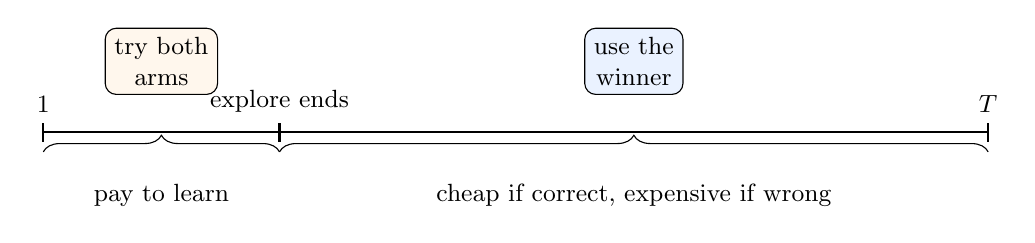
\begin{tikzpicture}[font=\small, >=Latex]
  \draw[thick] (0,0) -- (12,0);
  \draw[thick] (0,-0.12) -- (0,0.12) node[above]{1};
  \draw[thick] (3,-0.12) -- (3,0.12) node[above]{explore ends};
  \draw[thick] (12,-0.12) -- (12,0.12) node[above]{$T$};
  \draw[decorate, decoration={brace, amplitude=6pt}, yshift=-0.25cm] (0,0) -- node[below=8pt]{pay to learn} (3,0);
  \draw[decorate, decoration={brace, amplitude=6pt}, yshift=-0.25cm] (3,0) -- node[below=8pt]{cheap if correct, expensive if wrong} (12,0);
  \node[draw, rounded corners, fill=softorange, align=center] at (1.5,0.9) {try both\\arms};
  \node[draw, rounded corners, fill=softblue, align=center] at (7.5,0.9) {use the\\winner};
\end{tikzpicture}
\caption{Explore-then-commit separates learning and earning. The separation makes the analysis easy and exposes what later algorithms improve.}
\end{figure}

\section{Bounding the wrong commitment probability}

The algorithm commits wrongly if
\[
\widehat\mu_2\geq \widehat\mu_1.
\]
This event can happen only if at least one empirical mean makes a noticeable error.

Since
\[
\mu_1-\mu_2=\Delta,
\]
the midpoint between the two means is
\[
\frac{\mu_1+\mu_2}{2}=\mu_1-\frac{\Delta}{2}=\mu_2+\frac{\Delta}{2}.
\]
If both estimates are on the correct side of this midpoint, then arm 1 wins:
\[
\widehat\mu_1>\frac{\mu_1+\mu_2}{2}>\widehat\mu_2.
\]
Therefore, the wrong event implies at least one failure:
\[
\{\widehat\mu_2\geq\widehat\mu_1\}
\subseteq
\left\{\widehat\mu_1\leq \mu_1-\frac{\Delta}{2}\right\}
\cup
\left\{\widehat\mu_2\geq \mu_2+\frac{\Delta}{2}\right\}.
\]

For bounded rewards in $[0,1]$, Hoeffding's inequality says
\[
\Pp(\widehat\mu-\mu\geq \varepsilon)
\leq
\exp(-2m\varepsilon^2),
\]
and the same bound holds for downward deviations. With $\varepsilon=\Delta/2$,
\[
\exp\left(-2m\left(\frac{\Delta}{2}\right)^2\right)
=
\exp\left(-\frac{m\Delta^2}{2}\right).
\]
Using a union bound:
\[
\Pp(E_1\cup E_2)\leq \Pp(E_1)+\Pp(E_2).
\]
So
\[
\Pp(\widehat\mu_2\geq \widehat\mu_1)
\leq
2\exp\left(-\frac{m\Delta^2}{2}\right).
\]

\begin{proofbox}{Wrong commitment, line by line}
\[
\begin{aligned}
\Pp(\widehat\mu_2\geq\widehat\mu_1)
&\leq
\Pp\left(\widehat\mu_1\leq \mu_1-\frac{\Delta}{2}\right)
+
\Pp\left(\widehat\mu_2\geq \mu_2+\frac{\Delta}{2}\right)\\
&\leq
\exp\left(-2m\left(\frac{\Delta}{2}\right)^2\right)
+
\exp\left(-2m\left(\frac{\Delta}{2}\right)^2\right)\\
&=
2\exp\left(-\frac{m\Delta^2}{2}\right).
\end{aligned}
\]
\end{proofbox}

Plugging this into regret gives
\[
\E[\Reg_T]
\leq
m\Delta+2T\Delta\exp\left(-\frac{m\Delta^2}{2}\right).
\]

\section{What this simple algorithm teaches}

Explore-then-commit is not the algorithm one should trust in a serious system. Its value is pedagogical. It shows the main bargain.

If $m$ is small, the second term can be large: the learner may commit to the wrong arm. If $m$ is large, the first term is large: the learner wastes too many trials on a known bad arm.

\begin{plainbox}{The bargain}
Exploration is like paying rent for information. Too little rent and you stay ignorant. Too much rent and you never earn enough from what you learned.
\end{plainbox}

The next idea, optimism, improves this by not fixing the exploration budget in advance.

% ------------------------------------------------------------
\chapter{Optimism: Trust the Unknown Until It Disappoints You}

\section{The idea in one sentence}

Optimism is not positivity. It is a rule for action under uncertainty.

\begin{plainbox}{Optimism}
If an arm has not been tried much, allow it to look better than its current average. If it is truly bad, enough trials will shrink this allowance and remove it from serious competition.
\end{plainbox}

This is the idea behind UCB: upper confidence bound.

At time $t$, for each arm $a$, compute
\[
\text{index}_a(t)=\widehat\mu_a(t)+r_a(t),
\]
where $\widehat\mu_a(t)$ is the observed average and $r_a(t)$ is a confidence radius. Choose the arm with the largest index.

\[
A_t\in\argmax_a\left\{\widehat\mu_a(t)+r_a(t)\right\}.
\]

\begin{figure}[h]
\centering
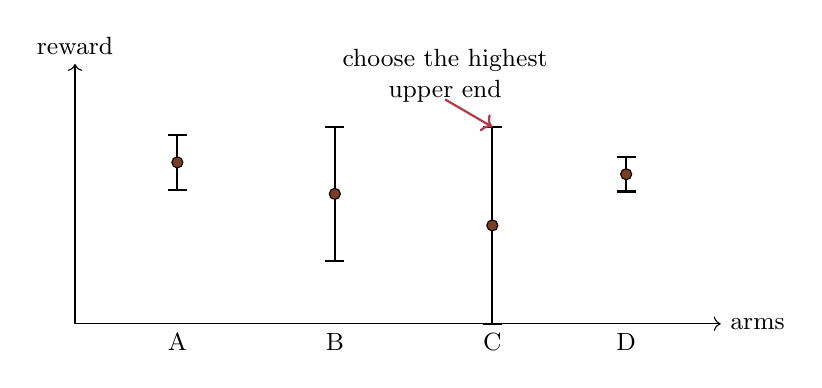
\begin{tikzpicture}[font=\small]
  \draw[->] (0,0) -- (8.2,0) node[right]{arms};
  \draw[->] (0,0) -- (0,3.3) node[above]{reward};
  \foreach \x/\m/\r/\lab in {1.3/2.05/0.35/A,3.3/1.65/0.85/B,5.3/1.25/1.25/C,7.0/1.90/0.22/D}{
    \draw[thick] (\x,\m-\r) -- (\x,\m+\r);
    \draw[thick] (\x-0.12,\m-\r) -- (\x+0.12,\m-\r);
    \draw[thick] (\x-0.12,\m+\r) -- (\x+0.12,\m+\r);
    \filldraw[fill=blogblue] (\x,\m) circle (2pt);
    \node[below] at (\x,0) {\lab};
  }
  \node[align=center, text width=2.7cm] at (4.7,3.15) {choose the highest\\upper end};
  \draw[->, thick, blogorange] (4.7,2.85) -- (5.3,2.5);
\end{tikzpicture}
\caption{UCB chooses the arm with the best plausible value, not necessarily the best current average.}
\end{figure}

\section{Where the radius comes from}

Let an arm be pulled $n$ times. Let its rewards be $Y_1,\ldots,Y_n$, each in $[0,1]$, with mean $\mu$. The empirical mean is
\[
\widehat\mu_n=\frac{1}{n}\sum_{i=1}^n Y_i.
\]
Hoeffding's inequality says
\[
\Pp\left(\widehat\mu_n-\mu\geq r\right)
\leq
\exp(-2nr^2).
\]
We want the right side to be a tiny number, say $t^{-4}$. So choose $r$ by solving
\[
\exp(-2nr^2)=t^{-4}.
\]
Now solve it slowly:

\begin{derivationbox}{Solving for the UCB radius}
\[
\begin{aligned}
\exp(-2nr^2)&=t^{-4}\\
\log\left(\exp(-2nr^2)\right)&=\log(t^{-4})\\
-2nr^2&=-4\log t\\
2nr^2&=4\log t\\
r^2&=\frac{2\log t}{n}\\
r&=\sqrt{\frac{2\log t}{n}}.
\end{aligned}
\]
\end{derivationbox}

Thus a natural confidence radius is
\[
r_a(t)=\sqrt{\frac{2\log t}{N_a(t)}}.
\]
It shrinks when the arm is sampled often. It grows slowly with time because the algorithm makes many decisions and we want confidence to hold across many of them.

\section{The good event}

Here is the event we want:
\[
\left|\widehat\mu_a(t)-\mu_a\right|
\leq
r_a(t)
\quad\text{for all arms and relevant times.}
\]
Call this event $G$. On $G$, every confidence interval contains its true mean.

Why can we hope $G$ holds? Because each individual failure is rare, and a union bound lets us add many rare failures.

\begin{proofbox}{Union bound in the UCB setting}
For one arm and one sample size $n$,
\[
\Pp\left(\widehat\mu_{a,n}-\mu_a>\sqrt{\frac{2\log T}{n}}\right)
\leq
\exp\left(-2n\cdot\frac{2\log T}{n}\right)
=T^{-4}.
\]
The lower tail is the same:
\[
\Pp\left(\mu_a-\widehat\mu_{a,n}>\sqrt{\frac{2\log T}{n}}\right)
\leq T^{-4}.
\]
Therefore
\[
\Pp\left(\left|\widehat\mu_{a,n}-\mu_a\right|>\sqrt{\frac{2\log T}{n}}\right)
\leq 2T^{-4}.
\]
There are at most $KT$ pairs $(a,n)$, so
\[
\Pp(G^c)
\leq
\sum_{a=1}^K\sum_{n=1}^T 2T^{-4}
=2KT^{-3}.
\]
\end{proofbox}

No mystery is hidden here. The good event is just the statement that all sample averages are close to their true means. The union bound is just the rule that if many bad things can happen, the chance that at least one happens is at most the sum of their chances.

\section{Why a bad arm eventually loses}

Let $a$ be a suboptimal arm. Its gap is
\[
\Delta_a=\mu_* - \mu_a>0.
\]
Suppose the good event $G$ holds and UCB chooses arm $a$ at time $t$. Since UCB chose $a$, its index must be at least the index of the best arm $*$:
\[
\widehat\mu_a(t)+r_a(t)
\geq
\widehat\mu_*(t)+r_*(t).
\]
On $G$,
\[
\widehat\mu_*(t)+r_*(t)\geq \mu_*.
\]
Also on $G$,
\[
\widehat\mu_a(t)
\leq \mu_a+r_a(t).
\]
Thus
\[
\widehat\mu_a(t)+r_a(t)
\leq
\mu_a+2r_a(t).
\]
Putting the inequalities together:
\[
\mu_*
\leq
\mu_a+2r_a(t).
\]
Therefore
\[
\Delta_a\leq 2r_a(t).
\]
Using $r_a(t)=\sqrt{2\log T/N_a(t)}$:
\[
\Delta_a\leq 2\sqrt{\frac{2\log T}{N_a(t)}}.
\]
Now solve for $N_a(t)$:

\begin{derivationbox}{A bad arm can be chosen only while its radius is large}
\[
\begin{aligned}
\Delta_a&\leq 2\sqrt{\frac{2\log T}{N_a(t)}}\\
\frac{\Delta_a}{2}&\leq \sqrt{\frac{2\log T}{N_a(t)}}\\
\frac{\Delta_a^2}{4}&\leq \frac{2\log T}{N_a(t)}\\
N_a(t)&\leq \frac{8\log T}{\Delta_a^2}.
\end{aligned}
\]
\end{derivationbox}

This is the entire UCB proof in one picture: a bad arm is played only while it can still hide behind uncertainty. Once its confidence interval is narrow enough, it cannot beat the best arm's lower reality anymore.

\section{The regret bound}

On the good event, each bad arm $a$ is pulled at most about
\[
\frac{8\log T}{\Delta_a^2}
\]
times after initialization. Its regret contribution is gap times count:
\[
\Delta_a\cdot \frac{8\log T}{\Delta_a^2}
=
\frac{8\log T}{\Delta_a}.
\]
Adding arms gives
\[
\E[\Reg_T]
\lesssim
\sum_{a:\Delta_a>0}\frac{\log T}{\Delta_a}.
\]

\begin{takeawaybox}
UCB is not a complicated formula. It is a disciplined way to say: try uncertain things while they could plausibly be good; stop trying them once the data have made that hope too expensive to believe.
\end{takeawaybox}

% ------------------------------------------------------------
\chapter{Sampling a Possible World}

\section{The Bayesian picture}

Optimism says: choose the arm with the best plausible upper value.

Posterior sampling says something lighter:

\begin{plainbox}{Posterior sampling}
Imagine one possible world consistent with the data. Act optimally in that imagined world. Repeat this every round.
\end{plainbox}

This is Thompson sampling. It is one of the cleanest ideas in sequential learning. It often looks almost too simple: keep a posterior distribution over the unknown rewards, sample from it, and choose the arm that is best under the sample.

\section{A coin-click model}

Suppose each thumbnail has an unknown click probability $\theta_a$. A click is $1$, no click is $0$:
\[
X_t(a)\sim\Ber(\theta_a).
\]
For each arm, start with a Beta prior:
\[
\theta_a\sim\Beta(\alpha_a,\beta_a).
\]
If the arm receives a click, increase $\alpha_a$ by one. If it receives no click, increase $\beta_a$ by one.

\begin{derivationbox}{Beta-Bernoulli update}
\[
\begin{aligned}
\text{prior density:}\quad
p(\theta)&\propto \theta^{\alpha-1}(1-\theta)^{\beta-1},\\
\text{one click:}\quad
p(1\mid \theta)&=\theta,\\
\text{posterior:}\quad
p(\theta\mid 1)&\propto \theta\cdot \theta^{\alpha-1}(1-\theta)^{\beta-1}\\
&=\theta^{\alpha}(1-\theta)^{\beta-1},\\
\theta\mid 1&\sim \Beta(\alpha+1,\beta).
\end{aligned}
\]
\[
\begin{aligned}
\text{one no-click:}\quad
p(0\mid\theta)&=1-\theta,\\
p(\theta\mid 0)&\propto (1-\theta)\theta^{\alpha-1}(1-\theta)^{\beta-1}\\
&=\theta^{\alpha-1}(1-\theta)^{\beta},\\
\theta\mid 0&\sim\Beta(\alpha,\beta+1).
\end{aligned}
\]
\end{derivationbox}

After $S_a$ clicks and $F_a$ no-clicks on arm $a$,
\[
\theta_a\mid\text{data}\sim\Beta(\alpha_a+S_a,\beta_a+F_a).
\]

\section{The decision rule}

At time $t$:
\[
\widetilde\theta_a(t)\sim\Beta(\alpha_a+S_a(t),\beta_a+F_a(t)),
\]
independently for each arm, and choose
\[
A_t\in\argmax_a \widetilde\theta_a(t).
\]

\begin{figure}[h]
\centering
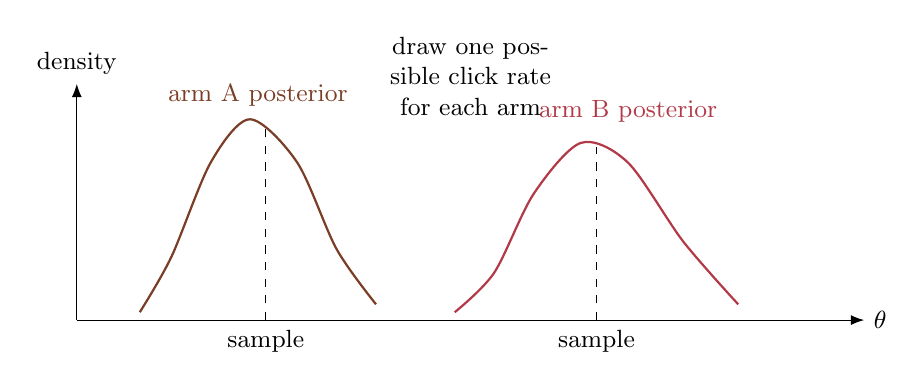
\begin{tikzpicture}[font=\small, >=Latex]
  \draw[->] (0,0) -- (10,0) node[right]{$\theta$};
  \draw[->] (0,0) -- (0,3) node[above]{density};
  \draw[thick, blogblue, smooth] plot coordinates {(0.8,0.1) (1.2,0.8) (1.7,2.0) (2.2,2.55) (2.8,2.0) (3.3,0.9) (3.8,0.2)};
  \draw[thick, blogorange, smooth] plot coordinates {(4.8,0.1) (5.3,0.6) (5.8,1.6) (6.4,2.25) (7.0,2.0) (7.7,1.0) (8.4,0.2)};
  \node[blogblue] at (2.3,2.85) {arm A posterior};
  \node[blogorange] at (7.0,2.65) {arm B posterior};
  \draw[dashed] (2.4,0) -- (2.4,2.5);
  \draw[dashed] (6.6,0) -- (6.6,2.2);
  \node[below] at (2.4,0) {sample};
  \node[below] at (6.6,0) {sample};
  \node[align=center, text width=3.7cm] at (5.0,3.1) {draw one possible click rate\\for each arm};
\end{tikzpicture}
\caption{Thompson sampling does not directly add a confidence bonus. It samples a plausible world and follows the best arm in that world.}
\end{figure}

\section{Why this explores}

If an arm has little data, its posterior is wide. A wide posterior occasionally samples a high value. That gives the arm chances to be tried. If the arm is bad, the failures push its posterior down and make such lucky samples rarer.

So the exploration is not manually scheduled. It emerges from uncertainty.

\begin{researchbox}{Classical paradigm: probability matching}
Thompson sampling chooses an arm with probability equal to the posterior probability that the arm is optimal. Arms are tried according to how believable their optimality is under current evidence.
\end{researchbox}

Let $A^*$ be the optimal arm under the unknown true parameter. Given the history $\calF_t$, posterior sampling satisfies
\[
\Pp(A_t=a\mid\calF_t)
=\Pp(A^*=a\mid\calF_t).
\]
This identity is the clean algebraic soul of Thompson sampling.

\section{The identity slowly}

Let $\theta$ be the unknown vector of arm means. Let
\[
g(\theta)=\argmax_a \theta_a.
\]
The true optimal arm is
\[
A^*=g(\theta).
\]
Thompson sampling draws
\[
\widetilde\theta\sim \text{posterior of }\theta\text{ given }\calF_t,
\]
and plays
\[
A_t=g(\widetilde\theta).
\]
Because $\theta$ and $\widetilde\theta$ have the same conditional distribution given $\calF_t$,
\[
\theta\mid\calF_t
\quad\overset{d}{=}\quad
\widetilde\theta\mid\calF_t.
\]
Therefore applying the same map $g$ preserves the conditional distribution:
\[
g(\theta)\mid\calF_t
\quad\overset{d}{=}\quad
g(\widetilde\theta)\mid\calF_t.
\]
Thus
\[
A^*\mid\calF_t
\quad\overset{d}{=}\quad
A_t\mid\calF_t.
\]
So for each arm $a$,
\[
\Pp(A^*=a\mid\calF_t)=\Pp(A_t=a\mid\calF_t).
\]

This proof uses no heavy probability. It says: if two hidden worlds are drawn from the same bag, then the winner in the first world and the winner in the second world have the same chance of being any given arm.

\section{Information accounting}

Many modern Thompson sampling analyses, including work in the broader line of information-ratio proofs, ask a simple question:

\begin{quote}
How much regret do we pay per unit of information gained?
\end{quote}

The technical details can become intricate, but the idea is almost everyday reasoning. If a trial is expensive but teaches a lot, it may be worth it. If a trial is expensive and teaches little, a good algorithm should avoid repeating it.

This way of thinking connects cleanly to recent theoretical work on Thompson sampling, best-arm identification with regret control, and multi-agent bandits, including work by Jin and collaborators \cite{jin2022expts,yang2024minimal,jin2024mamab}. The common flavor is not just to design a rule, but to prove that the rule pays for uncertainty in a controlled way.

% ------------------------------------------------------------
\chapter{Why This Toy Model Keeps Reappearing}

\section{Context changes the arms}

The homepage example was too simple: every visitor was treated the same. In practice, users arrive with context: time, device, language, past behavior, location, or topic preference.

A contextual bandit sees a context $x_t$, chooses an action $A_t$, and receives the reward of that action. The missing counterfactual remains:
\[
\text{observe }X_t(A_t,x_t),
\qquad
\text{miss }X_t(a,x_t),\ a\neq A_t.
\]
The setting becomes richer, but the wound is the same.

\begin{figure}[h]
\centering
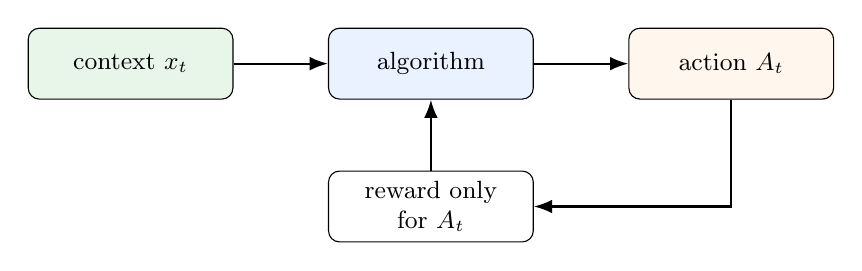
\begin{tikzpicture}[font=\small, >=Latex]
  \node[draw, rounded corners, fill=softgreen, minimum width=2.6cm, minimum height=0.9cm] (x) {context $x_t$};
  \node[draw, rounded corners, fill=softblue, minimum width=2.6cm, minimum height=0.9cm, right=1.2cm of x] (alg) {algorithm};
  \node[draw, rounded corners, fill=softorange, minimum width=2.6cm, minimum height=0.9cm, right=1.2cm of alg] (a) {action $A_t$};
  \node[draw, rounded corners, fill=white, minimum width=2.6cm, minimum height=0.9cm, below=0.9cm of alg, align=center] (r) {reward only\\for $A_t$};
  \draw[->, thick] (x) -- (alg);
  \draw[->, thick] (alg) -- (a);
  \draw[->, thick] (a) |- (r);
  \draw[->, thick] (r) -- (alg);
\end{tikzpicture}
\caption{Contextual bandits add side information before the action. They do not restore the missing outcomes of unchosen actions.}
\end{figure}

\section{Linear bandits: the geometry version}

In a linear bandit, each action has a feature vector $x_a\in\R^d$, and the mean reward is assumed to be approximately linear:
\[
\mu_a=x_a^\top\theta_*.
\]
The unknown object is now a vector $\theta_*$. Each action gives one noisy measurement of this vector in the direction $x_a$.

A helpful picture is this: learning a linear bandit is like trying to locate a hidden point in space by shining flashlights from different directions. Some directions reveal new information. Others repeat what is already known.

The UCB idea becomes geometric:
\[
\text{score}(x)=x^\top\widehat\theta+\beta\sqrt{x^\top V^{-1}x}.
\]
The first term is what we currently believe. The second term is how uncertain we are in direction $x$.

\begin{derivationbox}{Linear confidence in one line}
\[
\begin{aligned}
|x^\top(\widehat\theta-\theta_*)|
&=|\langle x,\widehat\theta-\theta_*\rangle|\\
&=|\langle V^{-1/2}x,V^{1/2}(\widehat\theta-\theta_*)\rangle|\\
&\leq \|V^{-1/2}x\|_2\cdot\|V^{1/2}(\widehat\theta-\theta_*)\|_2\\
&\leq \sqrt{x^\top V^{-1}x}\cdot \beta.
\end{aligned}
\]
\end{derivationbox}

The last inequality is just Cauchy-Schwarz plus a confidence ellipsoid. This is the geometric heart of linear UCB.

\section{Gaussian-process bandits: smooth unknown landscapes}

Sometimes actions are not a small list. They may be continuous: temperature in a lab, a hyperparameter, a drug dosage, a robotics controller, or a design choice. The reward function may be smooth but unknown.

Gaussian-process bandits model the unknown function as a random smooth landscape. The algorithm samples or optimizes where the landscape might be high, while learning the shape of the landscape from noisy evaluations.

The same old idea appears again:
\[
\text{mean prediction} + \text{uncertainty bonus}.
\]
For GP-UCB this takes the form
\[
A_t\in\argmax_{x\in\calX}\left\{m_{t-1}(x)+\sqrt{\beta_t}\sigma_{t-1}(x)\right\}.
\]
This line connects finite-armed bandits to Bayesian optimization, a major line of work including Srinivas, Krause, Kakade, and Seeger \cite{srinivas2010gpucb}, the Cambridge probabilistic modelling tradition \cite{ghahramani2015probabilistic}, and Oxford work on Gaussian-process global optimization \cite{osborne2009gp}.

\begin{figure}[h]
\centering
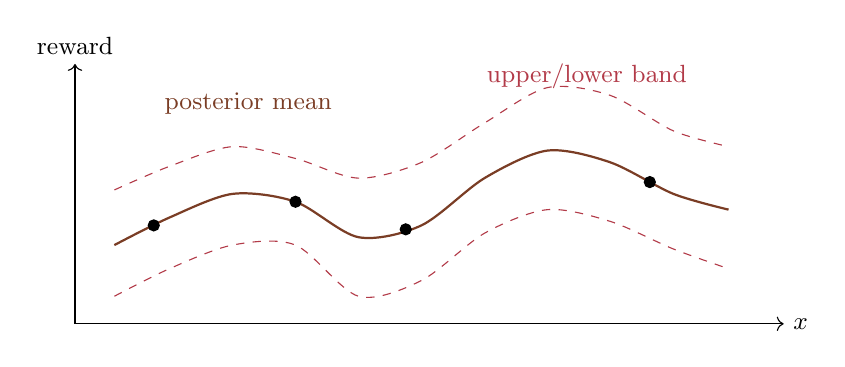
\begin{tikzpicture}[font=\small]
  \draw[->] (0,0) -- (9,0) node[right]{$x$};
  \draw[->] (0,0) -- (0,3.3) node[above]{reward};
  \draw[thick, blogblue, smooth] plot coordinates {(0.5,1.0) (1.2,1.35) (2.0,1.65) (2.8,1.55) (3.6,1.1) (4.4,1.25) (5.2,1.85) (6.0,2.2) (6.8,2.05) (7.6,1.65) (8.3,1.45)};
  \draw[dashed, blogorange, smooth] plot coordinates {(0.5,1.7) (1.2,2.0) (2.0,2.25) (2.8,2.1) (3.6,1.85) (4.4,2.05) (5.2,2.55) (6.0,3.0) (6.8,2.9) (7.6,2.45) (8.3,2.25)};
  \draw[dashed, blogorange, smooth] plot coordinates {(0.5,0.35) (1.2,0.7) (2.0,1.0) (2.8,1.0) (3.6,0.35) (4.4,0.55) (5.2,1.15) (6.0,1.45) (6.8,1.3) (7.6,0.95) (8.3,0.7)};
  \foreach \x/\y in {1.0/1.25,2.8/1.55,4.2/1.2,7.3/1.8}{\filldraw[fill=black] (\x,\y) circle (2pt);}
  \node[blogblue] at (2.2,2.8) {posterior mean};
  \node[blogorange] at (6.5,3.15) {upper/lower band};
\end{tikzpicture}
\caption{In GP bandits, the confidence interval becomes a band over a function. The old finite-arm picture survives, but the arms now live in a space.}
\end{figure}

\section{Reliable AI and the same old missing column}

The same obstruction appears in modern systems. A recommender only observes the item it showed. A tutoring system only observes the hint it gave. A medical decision support tool may only observe the outcome under the chosen treatment. An LLM steering policy only observes the response produced under the chosen prompt or intervention.

The names change. The missing counterfactual remains.

This is why bandits are not just a topic. They are a microscope. They strip sequential decision-making down to its smallest difficult piece.

% ------------------------------------------------------------
\chapter*{Epilogue: The Essence}
\addcontentsline{toc}{chapter}{Epilogue: The Essence}

The whole note can be compressed into a few sentences.

Supervised learning receives examples. Bandit learning creates examples by acting. Because only the chosen action is observed, the learner must spend some reward to buy information. Regret is the receipt for that purchase.

Explore-then-commit buys information on a fixed schedule. UCB buys it adaptively by giving uncertain arms temporary credit. Thompson sampling buys it by sampling possible worlds and acting according to their winners. Linear and Gaussian-process bandits carry the same ideas into structured spaces.

The deepest lesson is not a formula. It is a research habit: before designing an algorithm, ask what feedback is actually visible. Most of the mathematics follows from that one question.

\backmatter
\printbibliography[heading=bibintoc,title={References}]

\end{document}


